\chapter{Investigating the Intersection of Policing, Place, and Opioids}
%introduction 
% 1. brief contextualization of the opioid od crisis
% 2. role of place in driving od's
% 3. relationship between place, crime, and police
% 4. this may explain police involvment in ods, compared to other first responders 
% 5. but there is little research examining place based explanations of police involvement in od's

%Lit:
%Describe the role of nhood predictors predicting crime and opioid overdoses
%Described literature on why there may be variation in where PD and other first responders respond quicker too

% methods: figures of ods, property crime, violent crime, TPD/TFMR first administration, choropleth maps, then Andreson's S index, descriptive stats of block groups, ml logit looking at incident and nhood predictors for variation btween tpd and tfmr admins.

\section{\centering Introduction}
As opioid overdoses have increased exponentially over the last two decades, the police have increasingly assumed a more complex role in responding to the problem \parencite{quinn_most_2019, ray_national_2023}. In some cases they are involved in post-overdose outreach \parencite{formica_characteristics_2021,ray_national_2023} acting as a bridge to social services. While this is not outside of the police mission, it is a change from how police have traditionally handled substance use issues through arrests \parencite{cooper_war_2015}. Police officers being increasingly outfitted with naloxone -- an opioid antagonist -- means they can be effective in responding to and reversing opioid overdoses. However, there are concerns around police involvement in opioid overdoses. Namely, \textcite{lowder_twoyear_2020}'s findings suggest that individuals who overdosed and receive a police-response first (compared to emergency medical services; EMS), were more likely to be arrested. This increased criminalization requires further investigation, as \textcite{lowder_twoyear_2020} note. Particularly, investigating the incident and neighborhood factors that are associated with police being first on scene at an overdose is needed. Thus, it is crucial to understand how a police-first response to an opioid overdose is influenced by the communities that they serve.

The police tend to operate in communities marked by higher levels of calls for service, crime rates, and disadvantage (CITE). At the same time, public health issues such as suicide and substance use are spatially concentrated and overlap with communities marked by higher levels of crime as well \parencite{feldmeyer_community_2022, hibdon_use_2024}. Additionally, police officers tend to outnumber other first responders \parencite{lurigio_opioid_2018}. Because public safety issues, namely criminal activity, is a primary responsibility of the police, and because police officers are often actively patrolling and outnumber other first responders, police officers' response ecology differs from other first responders. In theory, the spatial convergence of public health and public safety issues position the police to respond quickly to opioid overdoses and provide immediate and effective life-saving care.

While the spatial overlap of crime and opioid overdoses is fairly well established \parencite{carter_spatial_2019, magee_dual_2022}, it is less clear if the police do in fact respond to opioid overdoses quicker in these neighborhoods. Because other public health issues can also overlap with crime and opioid overdoses, EMS or other first responders may be well suited to respond quickly as well. Additionally, it is possible that police operating in higher crime neighborhoods means that most of their time is spent handling higher priority issues (CITES). This would suggest that police response times to opioid overdoses may be delayed and other first-responders are better suited to respond first in these areas. Prior work that has looked at where police are more likely to administer naloxone tends to aggregate the total rate or count of naloxone administrations or responses to opioid overdoses for police \textit{and} EMS/Fire. This research suggests that, together, police and EMS naloxone administrations do concentrate geographically \parencite{heavey_descriptive_2018}. Other work that has attempted to investigate spatial variation in responsiveness between first-responders indicates that police officers may be more likely to be first on scene at an overdose in rural areas \parencite{wood_overdose_2021}. However, there are no studies that investigate the spatial variation between first responders at more granular geographic areas like the block group, a proxy for neighborhoods. This is an important avenue as it will shed light on when and where individuals are more likely to receive a police-first response at an opioid overdose.

The present study seeks to address this gap in the literature. Using Tempe Fire and Medical Rescue (TFMR) calls for service data I investigate the spatial variation in police administering naloxone first and TFMR administering naloxone first. I use a spatial point pattern test to first descriptively assess if there is variation in where police and TFMR are administering naloxone first across neighborhoods in Tempe, Arizona. Then, because of the nested structure of the data, I employ mixed-effects regression models to assess the incident- and neighborhood-level predictors of police and TFMR administering naloxone first. The findings have implications for policy that guides police discretion and decision-making at opioid overdoses, reinforces the need for inter-agency communication and collaboration, and the need for community-level programs to expand accessibility of naloxone for community members.

\section{\centering Literature Review}

\subsection{Place, Crime, and Opioid Overdoses}

Early geographical work of the 1800s inspired the contemporary Chicago school which emerged in the early 20th century. The Chicago school is a sociological perspective that explains how the structure of urban life influences outcomes. In one of the earliest tests of the role of urban structure and crime, \textcite{shaw_juvenile_1942} investigated why delinquency was unevenly distributed throughout the city. They found that neighborhoods that were socially disorganized – high levels of poverty, racial heterogeneity, and residential instability – experienced higher delinquency rates. \textcite{shaw_juvenile_1942} finding indicated that delinquency was not solely associated with individual-level characteristics, but that structure played a role as well. These findings led to the development of social disorganization theory which suggests that there are neighborhood-level characteristics that influence juvenile delinquency rates regardless of the individual characteristics of those in the neighborhood. One of the primary mechanisms used to explain this finding is that the formation of social ties is hindered in socially disorganized neighborhoods. The systemic model, proposed by \textcite{kasarda_community_1974}, places an emphasis on the social connections between community members \parencite{bursik_jr_economic_1993, bursik_systemic_2000}. Specifically, neighborhoods with strong ties between community members can convey norms, values, and expectations of conduct for the neighborhood. The transmission of these norms and values produces a greater capacity for informal social control among community members \parencite{kornhauser_social_1978}. However, the presence of disadvantage, residential instability, and ethnic heterogeneity can hinder the development of informal social controls. Because there is an inability to develop strong informal social control mechanisms in neighborhoods marked by disadvantage, deviance and other forms of criminal activity can go unthwarted. In one of the first full tests of social disorganization theory, \textcite{sampson_community_1989} showed that there was an indirect effect of neighborhood-level structural characteristics on crime and that the strength of networks among community members mediated the relationship. Contemporary work has continued to support this finding showing the impact of structural characteristics and the role of community ties play across jurisdictions \parencite{bursik_systemic_2000, levy_triple_2020, sampson_great_2012, sampson_neighborhoods_1997}.

Another ecological theoretical framework for explaining the association between community-level characteristics and crime is the macro-level strain theory proposed by \parencite{agnew_robert_general_1999}. Agnew suggests that the differential distribution of crime across communities is not solely a product of weak informal social controls but also a product of the strain producing characteristics in these communities that either blocks individuals’ goals, produces a feeling of deprivation, introduces negative stimuli, or removes positive stimuli. There is also a network effect wherein individuals who interact with other highly strained individuals that become strained themselves. Communities with strain producing characteristics select strained individuals, particularly for those who are facing economic hardships. These individuals move into the deprived community and are confined to the community because of their inability to relocate. This then leads to community-level differences in crime rates because of the heightened likelihood of a criminal response to the strain experienced in the given neighborhood.

Yet, tests of \textcite{agnew_robert_general_1999} model are relatively limited, particularly at the neighborhood level. Of the research that has been done at the neighborhood level, findings have highlighted the role of strain and its impact on community crime rates \parencite{antunes_social_2022, warner_strain_2003}. This research indicates that strain does play a role in the production of crime rates at the neighborhood level. \textcite{warner_strain_2003} show that the role of informal social controls become statistically non-significant while community-level strain is significantly associated with violence. \textcite{antunes_social_2022} report similar findings in that community level strain, exposure to violence, and youth violence are associated even when controlling for collective efficacy. 

Importantly, the same macro-level process of social disorganization theory and macro-level strain theory that are associated with crime are also relevant for drug use and overdoses. Community-level characteristics that have been found to be associated with overdoses and overdose mortality include higher levels of poverty, ethnic heterogeneity, lower home ownership rates, and low educational attainment \parencite{chichester_pharmacies_2020, galea_income_2003, hannon_neighborhood_2006, ford_neighborhood_2017}. \textcite{ford_neighborhood_2017} show that social disorganization, a lack of social capital, and low social participation are predictive of adolescent opioid misuse. \textcite{winstanley_association_2008} also find the same relationship between social capital - measured as participation in community based groups -- and reported opioid dependence. This could suggest that higher levels of social capital indicate greater levels of connectedness with community, family, and school. These findings indicate that stronger ties and social integration is associated with lower levels of reported opioid use. Social connectedness likely improves the ability for community members to enact informal social controls and discourage drug use. 

Additionally, \textcite{feldmeyer_community_2022} notes that structural factors, which include higher opioid prescription rates, population decline, poor community health, and the loss of manufacturing jobs are associated with higher levels of overdoses. \textcite{feldmeyer_community_2022}'s findings are in line with the deaths of despair argument proposed by \textcite{case_rising_2015, case_mortality_2017}. Specifically, the same ecological characteristics are associated with overdose deaths and suicides. \textcite{feldmeyer_community_2022} extend this to show some overlap with homicides as well. In a more recent article looking at drug overdoses in Passaic County, New Jersey from 2015-2019 at the block-group level, \textcite{piza_drug_2023} finds that one of the strongest predictors of drug overdoses is concentrated disadvantage. 

The empirical work investigating the association between structural variables and opioid overdoses suggest that weakened social controls (i.e., lower home ownership rates, population decline, disadvantage) and strain (e.g., loss of employment) influence opioid overdose rates. As discussed above, the formation of ties is important for informal social control. Disadvantage, population decline, and lower homeownership rates are neighborhood characteristics that hinder the formation of social connections which reduces the capacity to develop informal control mechanisms. When informal social control is present, members of a community may discourage opioid use resulting in either less use or potentially less risky use. Also, unemployment and the loss of manufacturing jobs has been found to be associated with elevated opioid overdose rates. This is particularly true for the Appalachian region of the US where many hard labor jobs have become obsolete \parencite{mclean_theres_2016}. This association suggests there is a relationship between strain and opioid overdoses. Particularly for communities facing loss of employment opportunities and economic decline. Individuals may be strained because of their inability to achieve monetary goals and are unable to relocate given a variety of reasons including their economic situation. Communities facing economic hardships produce strain and retain strained individuals, which then leads to various forms of coping which could be opioid usage \parencite{monnat_factors_2018, monnat_contributions_2019}. While these findings suggest that policies should be implemented at the macro-level to address disadvantage, economic decline, and job loss to help facilitate the development of informal social control and reduce strain, there is a practical implication of this overlap between macro-level and neighborhood-level characteristics, crime, and opioid overdoses. Namely, the potential for police to be the first-responder at an opioid overdose given that they are also unevenly distributed throughout a city in areas marked by a higher volume of calls for service to crime-related incidents.

\subsection{Place and Policing}

Police work is often tied to space and time \parencite{fyfe_police_1991}. Police patrol and activity often reflects local crime trends and areas marked by disadvantage. Across cities, crime – particularly violent crime – tends to be concentrated in neighborhoods characterized by socioeconomic disadvantage \parencite{peterson_divergent_2010}. Because of this spatially concentration, police are likely to be situated in these areas frequently \parencite{engel_race_2012, mitchell_criminal_2011}. Deploying police resources based on need – defined as volume of calls for service – is the underpinning of the “deployment hypothesis” (but see \cite{alexander_war_2010, beckett_penal_2010}). Police departments have attempted to maximize the utility of their limited resources by having officers focus on high-crime areas \parencite{skogan_fairness_2004, weisburd_reforming_2003}. 

In line with the deployment hypothesis, hot spots policing has gained traction as a way to reduce various offense types such as violent, property, disorder, and drug offenses \parencite{braga_hot_2019}. Hot spots policing is a catch all term that captures police presence at micro-places that experience high levels of crime. What police officers do in these crime hot spots varies (e.g., increased number of officers, mere presence, problem oriented policing). Regardless, this approach to reducing crime is based on the law of crime concentration which suggests that crime concentrates among a small percentage of street segments across a given city \parencite{braga_benefits_2017, weisburd_law_2015}. Because of this law of crime concentration and the neighborhood-level characteristics that produce this spatial fact, police resources tend to be clustered.

Police officers being spatially concentrated suggests they may be better positioned to respond to overdoses quicker in places and for populations that may differ from other first-responders, given their availability and patrolling patterns. This is an important aspect of police work that is often overlooked when thinking about their role in responding to public health issues such as the opioid overdose crisis. It has been shown that although there is overlap between police and EMS data, though there is some spatial dissimilarity pertaining to violence and drug activity \parencite{hibdon_concentration_2017, hibdon_going_2021}. Likewise, police officers may be able to reach overdose incidents prior to EMS or the fire department which could be indicative of a quicker response time in these areas \parencite{pourtaher_naloxone_2022, white_leveraging_2022}. Debates about the role of the police responding to opioid overdoses typically embody a philosophical argument or one that focuses on iatrogenic effects of the police involvement \parencite{doe-simkins_whose_2022, michaud_therapeutic_2023, van_der_meulen_thats_2021}. However, this spatial component of police work as it relates to the opioid overdose crisis suggests the police may be able to administer naloxone and act as a conduit to services in areas where other first responders may infrequently respond to or are delayed in responding. 

\subsection{Policing Opioid Overdoses}

Opioid overdoses are very clearly a police problem, but there are only a handful of studies that examine drivers of the police response. In fact, there is some research that suggests the police may be more likely to respond first to an overdose in rural areas \parencite{wood_overdose_2021}. \textcite{pourtaher_naloxone_2022} also find that police are frequently first on scene at an overdose in the state of New York. In rural areas, resources for other first-responders may be insufficient and response times may be delayed which may explain this finding. Moreover, in Tempe, Arizona, when police respond to a suspected opioid overdose, they are frequently first on scene \parencite{white_leveraging_2022}. But what contextual factors are associated with police arriving first at an opioid overdose? This question has yet to be explored thoroughly, and as \textcite{lowder_twoyear_2020} notes, it is an important empirical question because it highlights when and where individuals who overdosed are more likely to be arrested. It also highlights areas where police discretion can be better utilized to connect individuals to services such as substance use treatment.

At the incident-level, the 911 call description may also influence who responds first. For instance, \textcite{atkins_disparities_2024} show that describing an overdose event as a "non-overdose" was more prevalent when the victim was Black or a female. The authors suggest this could be due to a fear of police response and the potential for an arrest. Prior work has highlighted this fear is prevalent in Black communities \parencite{wagner_post-overdose_2019} and that the general fear of arrest can deter calling 911 \parencite{van_der_meulen_thats_2021}. Moreover, in communities where drug use and specifically opioid use is more prevalent, this avoidance of using certain terminology could have an influence in the aggregate as some harm reduction organizations have advocated for using other terminology than "overdose" when calling 911 to avoid a police response \parencite{zagorski_how_2021}.

However, there is essentially no research on the predictors of police responding first to opioid overdoses outside of the urban/rural divide. It has only been discussed from a theoretical perspective. The present study seeks to address this gap in the literature. 

\section{Current Study}

I am interested in examining if there is a) spatial variation in where police administer naloxone first at the scene of an opioid overdose, and b) why this variation exists. To reiterate, there is a paucity of research in this area. Despite the some research pointing to an overlap of opioid overdoses and violent crime, there is little known about how this overlap may be associated with a police-first response to opioid overdoses. Moreover, there are other incident-level and neighborhood-level characteristics that may be associated with this outcome as well that have yet to be investigated. To evaluate the incident- and neighborhood-level characteristics of police administering naloxone first, I investigate two research questions:

1) Is there spatial variation, at the block group, in where police administer naloxone first at the scene of an opioid overdose? 

\begin{flushleft}
\(H1_a\): Police administering naloxone first at an opioid overdose incident will vary spatially across block groups. 
\end{flushleft}

2) Why is there spatial variation in where police are more likely to administer naloxone across block groups? 

\begin{flushleft}
\(H2_a\): The violent crime rate at the block group will be associated with police administering naloxone first at an opioid overdose incident.
\end{flushleft}

To answer these research questions, I use administrative data from Tempe Fire and Medical Rescue (TFMR) that contains calls for service to opioid related incidents. Importantly, there is an indicator of who administered naloxone prior to TFMR response. This allows me to identify which incidents received a police-first response and naloxone administration\footnote{In Tempe, TFMR responds to a larger call volume of opioid overdoses. Through communication with a TFMR analyst, police are on scene at an opioid overdose approximately 40\% to 50\% of the time. Of those, there is a subset where they are on scene first, according to \textcite{white_leveraging_2022}, they are on scene first frequently.}-- see below for a thorough description of the data. To answer the above research questions, I employ a spatial point pattern test to assess spatial variation in where police and TFMR are administering naloxone first. Second, I employ mixed-effects logistic regression models with month and year fixed effects to control for unobserved time varying confounders (e.g., seasonality, COVID-19, staffing shifts) to assess incident-level and block-group predictors of when and where police are more likely to administer naloxone first.

\section{Methods}
\subsection{Setting}

Since 2020 the Tempe Police Department (TPD) has been involved in a collaborative effort with a social services organization – La Frontera EMPACT – to reduce opioid overdose fatalities in Tempe, Arizona. This project, called the Tempe First-Responder Opioid Recovery Project, is funded by the Substance Abuse and Mental Health Services Administration (SAMHSA). The project trained and outfitted Tempe officers with naloxone in January of 2020 and created a 24/7 crisis hotline which officers contacted following an overdose incident to initiate a response from a peer navigator (e.g., social outreach worker). Within days of the incident the peer navigator meets with the overdose survivor and their family/friends to provide information regarding potentially useful services (e.g., counseling, drug rehabilitation, housing information, transportation, etc.). Tempe officers have responded to more than 300 overdose incidents during the project. They have administered naloxone over 250 times in which it aided in a successful reversal of opioid overdose symptoms, and they have contacted the 24/7 crisis hotline approximately the same number of times. 

\subsection{Data}
The original data set from TFMR contained 3,257 calls for service to an opioid related incident from January 2017 through November 2023. Data on TFMR calls for service to opioid related incidents can be pulled from \href{https://data.tempe.gov/datasets/2daeeafd2741494c8294ca415e5a793e_0/explore?location=33.398962%2C-111.931850%2C11.94}{Tempe.gov}.\footnote{Through a contact at TFMR I was able to obtain other variables -- in addition to the public dataset -- such as the dispatched complaint and whether it was a fatal or nonfatal overdose.} I then geocoded this data set in \texttt{R} using the package \texttt{tidygeocoder} where I specified ArcGIS services as the method for geocoding.\footnote{The geocoding process provides a score that captures how closely an observation matches an address. It ranges from 0 to 100. Of the 3,257 opioid overdose calls for service, the lowest score in the dataset was 79.0\% and overall, there was a mean matching score of 98.6\%.} I then spatially clipped the incident data to a Tempe boundary shapefile (n = 3,207). 

Next, I used the \texttt{tidycensus} package in \texttt{R} where I specified the specific block group socio-demographic variables for the analysis. I used the \texttt{getacs} command to obtain 5-year estimates (2018-2022) for block groups in Tempe, Arizona -- the specific variables will be discussed below. Then, I remove observations where the block group total population estimate is 0 (n = 3,143) -- this also drops 2 block groups (n = 115). Lastly, I remove observations prior to 2020 because the Tempe police department did not carry naloxone prior to 2020, and I drop observations in November of 2023 because the TFMR calls for service data was not a full month of reporting (n = 2,000). 

The offense data is pulled from \href{https://data.tempe.gov/datasets/1563be5b343b4f78b1163e97a9a503ad_0/explore?location=32.279019%2C-112.767075%2C7.97}{Tempe.gov}. The original dataset includes 320,991 observations. I began by limiting the dataset to the pertinent time period (Jan 2020 - Oct 2023; n = 102,681). I then specified three particular crime categories: violent crimes, property crimes, and drug offenses -- these specific categories will be described below. Then, I spatially clipped the offense data to the Tempe boundary shapefile (n = 101,534). 

\subsection{Dependent Variable}
There are two primary dependent variables for the present study: First, a dichotomous variable indicating whether law enforcement administered naloxone first at the scene of an opioid overdose. The final sample includes 288 observations (14.40\%) where law enforcement administered naloxone. There are 1,712 observations (85.60\%) where naloxone was either not administered at all, or naloxone was administered by someone other than law enforcement (e.g., layperson, TFMR, Unknown). The second dependent variable is a dichotomous variable indicating whether TFMR administered naloxone first (n = 665; 33.25\%) compared to all other outcomes (n = 1,335, 66.75\%; e.g., no administration, PD, layperson, etc.\footnote{As a sensitivity check I collapse this outcome variable on law enforcement and TFMR only. This results in 288 law enforcement administrations (30.22\%) and 665 TFMR administrations (69.78\%). This changes the reference category to more specifically assess variation between these two first-responders. The results do not change.}

\subsection{Independent Variable}
The primary independent variable of interest is the violent crime rate per 1000 residents at the block group. This variable is captured by summing incidence of homicide, manslaughter, aggravated assault, robbery, and burglary with force, dividing by the ACS 5-year population estimate and multiplying by 1000.

I control for both incident level and block group level predictors. At the incident-level I control for the initial dispatch complaint. This variable in it's original form has 31 different entries. I code them into a categorical variable that has six values.\footnote{See Appendix A Table 1 for how the variable was coded.} I separate them into \textit{overdose/poisoning}, \textit{health/medical related}, \textit{accidental injury}, \textit{public safety related}, \textit{mental health related} and \textit{other}. I also control for the sex of the individual (= 1 for female [male = 0]).\footnote{At the incident level, race is not included in the dataset. I discuss this in the limitations section. I do run supplemental models including if the individual was homeless and I include the age of the individual (reported as an age range). There is associated missingness with these variables, particularly for homelessness. Nonetheless, the main results do not change.} At the block group level, I control for drug offense rate,\footnote{Comprised of drug paraphernalia, possession/sell/manufacture of narcotics, and possession/manufacture of prescription drugs offenses.} opioid overdose rate logged, and a series of spatial lags calculated using the spatial weight matrix (\textit{W}) to account for nearby block groups violent crime, drug offenses, and opioid overdose incidents. Additionally, I control for the percentage of residents that are unemployed, non-Hispanic Black, non-Hispanic White, and Hispanic. I also control for the percent of land that is residential \footnote{This was calculated by using the \texttt{osmdata} package in \texttt{R} that allows for the pulling of specific land use features (e.g., bus stops, liquor stores, parks, residential land, etc.). Pulling this data provided a calculation for how much residential land was in Tempe, Arizona. Then, I spatially clipped this to the block group, where I then calculated the percent of residential land by dividing the land use that was residential by the total land in the block group, then multiplying by 100.} and the percent of owner occupied units. Lastly, I incorporate month and year fixed effects to account to time-varying confounders such as seasonality, impacts of COVID-19, and broader year-to-year shifts that may capture changes in employment levels.\footnote{As a sensitive check I also incorporate day of month fixed effects to account for potential variation across days and weeks, the results do not change.}

\subsection{Analytical Sample}
The final sample includes 2,000 calls for service to opioid overdose incidents from January 2020 through October 2023, nested within 115 block groups in Tempe, Arizona.

\subsection{Analytical Plan}
\subsubsection{Spatial Point Pattern Test}

First, to descriptively assess the spatial variation in TPD and TFMR naloxone administrations I employ a spatial point pattern test \parencite{andresen_testing_2009}. This approach compares the pattern of two (or more) outcomes across spatial units (e.g., cell grids, blocks, block groups, police precincts, etc.). It has been applied in a variety of contexts such as crime concentration, stability in crime over time, and others \parencite{andresen_crime_2017, ha_spatial_2020, ratcliffe_detecting_2005}. Specifically related to the present study, I am interested in understanding which neighborhoods experience a higher volume of TPD administering naloxone first on scene at an opioid overdose compared to TFMR. Thus, I have two outcomes of interest to compare spatially. 

The spatial point pattern test works by first identifying which outcome is the base data and which is the test data. Here, the TFMR naloxone administrations are the base data and the police administrations are the test data. Then, 85\% of the test data is randomly sampled (with replacement) and undergoes Monte Carlo simulations (n = 200). Next, the percentages of points identified within each neighborhood can be ranked which is then used to remove the top 2.5\% and bottom 2.5\%. This allows for the creation of a 95\% confidence interval around the percentage of the points in each neighborhood. The base data is finally compared to the test data. If the base data falls within the confidence interval, then the two spatial point patterns are similar \parencite{andresen_testing_2009}.

The spatial point pattern analysis can be represented as such:

\[
    S = \frac{\sum_{i=1}^n S_i}{n}
\]

\noindent Where \(n\) is the number of block groups and \(S_i\) is equal to one if the point patterns are similar for block group \(i\). This then produces two \(S\) values. A global \(S\) and robust \(S\). The former refers to a similarity index for all block groups even if the test data was not observed in the spatial units. The latter, however, limits the similarity index to block groups with at least one observation from the test data. 

\subsubsection{Mixed-effects Logistic Model}
To examine why there may be spatial variation in where police and TFMR are administering naloxone first, I employ mixed-effects logistic regression models to handle the nested structure of the data. Specifically, opioid overdose incidents nested within block groups. This allows me to have a random intercept for each block group, and to model incident and block group predictors simultaneously. The equation for this model is as follows:

\[
\text{logit}\left(P(Y_{ij} = 1)\right) = \beta_0 + \sum_{k} \beta_k X_{ij} + \delta_m \text{Month}_{ij} + \lambda_y \text{Year}_{ij} + u_j
\]

\noindent Where \(P(Y_{ij} = 1)\) represents the probability that police or TFMR administer naloxone first at incident \(i\) in block group \(j\). Then, \(\text{logit}(P)\) represents the log odds of police or TFMR administering first. \(\beta_0\) is the intercept and \(\sum_{k} \beta_k X_{ij}\) represents the sum of all fixed effects incident and block group predictor variables. \(\delta_m \text{Month}_{ij}\) and \(\lambda_y \text{Year}_{ij}\) represent month and year fixed effects, respectively. Lastly, \(u_j\) represents the random intercept of block group \(j\).

\section{Results}

Figure 1 depicts the results from the spatial point pattern analysis. Visually, it is clear that TFMR administering naloxone first is less concentrated and more prevalent in Southern Tempe (represented by the blue block groups). The standard \textit{S}-index is .378 and the robust \textit{S}-index is .327 (see table 2). To reiterate, an \textit{S}-index of 1 indicates perfect similarity and 0 perfect dissimilarity. However, \textcite{andresen_area-based_2016} notes that there is not a statistical test to determine similarity or dissimilarity. The general threshold that is used in the spatial point pattern test to identify similar data points is .80. Though, this is not a binary distinction. Both similarity indices in the present study range from .327 to .378 which suggests that there is spatial variation in where police are administering naloxone first compared to TFMR thus the first null hypothesis can be rejected. This informs the next set of analyses because it suggests that there are potential neighborhood characteristics that are associated with this variation where police are administering naloxone first compared to TFMR.

Table 2 presents the results from the main mixed-effects logistic regression models. Police were less likely to administer naloxone first in neighborhoods with higher violent crime rates (OR = 0.997 [.996, .998]). Additionally, police were less likely to administer naloxone first when the initial call for service was described as a health/medical issue (OR = .684 [.507,.920]), a mental health issue (OR = .391 [.241, .6320]), and other (OR = .649 [.4685, .898] compared to an "overdose/poisoning" description. Percentage of owner occupied units is negatively associated with police administering naloxone first (OR = .978 [.960, .995]). On the other hand, there were two neighborhood predictors that were associated with higher odds of a police naloxone administration: drug offense rate (OR = 1.007 [1.004, 1.010]) and percent non-Hispanic Black (OR = 1.025 [1.011, 1.039]).

The violent crime rate in the neighborhood was associated with TFMR being more likely to administer naloxone first (OR = 1.001 [1.000, 1.002]), though for both police and TFMR these are small substantive differences. TFMR was more likely to administer naloxone first when the intial call for service was described as a health/medical issue (OR = 1.326 [1.013, 1.734]), a mental health issue (OR = 1.998 [1.396, 2.858]), and other (OR = 2.948 [ 2.152, 4.038] compared to an "overdose/poisoning" description. Lastly, drug offense rate was associated with a lower likelihood of TFMR administering naloxone first (OR = .994, [.991, .997]). Figure 2 provides a visualization of the statistically significant coefficients. Panel A includes neighborhood predictors and panel B contains coefficients for dispatch type.

Table 3 provides the results of a supplemental mixed-effects logistic regression model focused solely on police administering naloxone first compared to TFMR administering naloxone first. More specifically, the reference group is now TFMR administering naloxone first. The results do not substantively change from table 2 although the association between percentage owner occupied units is now marginally significant (\textit{p} < .10). See figure 3 for a visualization of the coefficients.

\section{\centering Discussion}
% contextualize
The present study uses spatial point pattern testing and mixed-effects logistic regression models to investigate spatial variation in where police and TFMR are administering naloxone first at opioid overdose incidents. There is a paucity of research examining spatial variation in police and other first responders involvement in opioid overdoses, particularly for smaller geographical areas. To my knowledge, the present study is the first to do so at a more granular geographical level. 

% interpret
The results from the spatial point pattern analysis suggest that that there is variation in where police officers are administering naloxone first compared to TFMR. Although this test does not tell use why this variation exists, prior research that discusses variation in hot spots of drug activity for PD and EMS data \parencite{hibdon_concentration_2017, hibdon_going_2021} and the deployment of police to areas with higher levels of calls for service and crime \parencite{engel_police_2003} provides a foundation as to why police may be administering in different areas. The \textit{S}-index in the present study is similar to \textcite{hibdon_concentration_2017}'s similarity index where they found that EMS and PD calls for drug activity overlapped between 24\% and 36\% of the time, though, they were looking at street segments and intersections. 

The results from the mixed-effects logistic regression models provide some context for when and where police are more likely to administer naloxone first. And although the estimates are statistically significant, substantively, they are small odds ratios. Specifically, violent crime rate is associated with a 0.3\% decrease in the odds of police administering first. One explanation for this relationship is that in neighborhoods with higher levels of violent crime, police resources are spread thin handling serious crimes and are thus less likely to respond to opioid overdoses which positions TFMR to be the primary first-responder for these calls for service in these particular neighborhoods.

Regarding the initial call dispatch, compared to an overdose description, police officers are less likely to administer naloxone first when it is health or medical related, mental health related, or other. This makes sense as health related calls are going to be prioritized by TFMR and will be of lower priority for police. This aligns with the research conducted by \textcite{seim_bandage_2020}. Specifically, in some instances police and EMS prioritize the same call yet there is still variation in which calls are prioritized which can lead to variation in the first responder on scene \parencite{hibdon_concentration_2017}.

Additionally, the drug offense rate in the neighborhood was associated with an increase in the odds of police administering naloxone first. It may be the case that neighborhoods marked by drug offenses alert police officers to these neighborhoods for potential future drug activity. Prior work indicates that police can reduce drug-related incidents through problem solving \parencite{mazerolle_street-level_2007}. In Tempe, police officers may be patrolling these neighborhoods which positions them to respond and administer naloxone quickly when there is an overdose. 

% perc owner occ units
Also, the percent of owner occupied units in the neighborhood was associated with a decrease in the odds of police administering naloxone first in table 1 but a marginally significant decrease in table 2. This indicates that police are more likely to administer naloxone first in neighborhoods with higher-levels of renter-occupied units or vacant units. Together, renter-occupied and vacant units indicate lower levels of informal social control and more opportunity for criminal activity and drug use \parencite{feldmeyer_community_2022, hannon_neighborhood_2006}. On the other hand, homeownership tends to indicate higher levels of informal social control and collective efficacy \parencite{sampson_neighborhoods_1997} which signals residents' willingness to intervene in devious acts. The finding indicates that police officers may be acting as a formal control mechanism in areas with lower owner occupied units which positions them to respond in a timely manner and administer naloxone.

% black
Lastly, the percent of non-Hispanic Black residents in the neighborhoods was associated with an increase in the odds of police administering naloxone first. The empirical literature on policing, race, and place, suggests that police officers tend to operate in neighborhoods marked by disadvantage which are disproportionately comprised of racial/ethnic minorities which has been associated with racially biased outcomes \parencite{fagan_street_2000}. However, in the context of this study, the outcome being naloxone administration indicates that police officers are quickly responding to provide life-saving care. This finding highlights the interplay between how police resources are distributed across the city and the potential for delayed emergency medical responses in marginalized communities. 

\subsection{Limitations}
There are some limitations of the present study that are worth mentioning. First, the data is derived from TFMR which are citizen-initiated calls for service. Not all opioid overdoses are called in and thus the present data are likely under counts of the true frequency of opioid overdoses. Second, at the incident-level there is no race variable which hinders the study's ability to assess \textit{who} police are administering naloxone to first. Third, the analysis is cross sectional and lacks the ability to speak to the temporal ordering of the relationships between the variables. Lastly, the study focuses on Tempe, Arizona and likely lacks generalizability to other cities. However, future research should investigate the spatial variation in responsiveness to opioid overdoses in other jurisdictions at the neighborhood level to help inform first-responders and communities better address the opioid overdose crisis.

\subsection{Implications}

The findings have some implications. First, violent crime rates at the neighborhood being associated with a lower likelihood of police administering naloxone first may indicate that police officers are spread thin in these neighborhoods. If this is what is driving the relationship, collaboration between the police department and TFMR should be developed to enhance data sharing to facilitate more effective responses in neighborhoods where the police department may be resource deficient. This is particularly true if a police response is generally quicker than TFMR but is hindered in neighborhoods marked by higher rates of violent crime. This will ensure that individuals experiencing an opioid overdose are receiving a timely response in these neighborhoods. 

Second, the complex mission of the police, specifically the conflict between public safety and public health roles, must be clearly delineated in policy when it comes to addressing the opioid overdose crisis \parencite{del_pozo_beyond_2021}. For instance, in both communities with a larger share of Black residents and communities marked by higher rates of drug offenses, it is critical to approach the opioid overdose itself from a public health stance. This should entail prioritizing the health of the individual and connecting the individual to potentially useful services. In Tempe, this is the priority with the Tempe ORP in place. A punitive approach -- prioritizing arrests -- may hinder relationships with community members \parencite{van_der_meulen_thats_2021}, exacerbate racially biased outcomes \parencite{kochel_effect_2011}, and be detrimental to the overdose victim by increasing their risk of a future overdose \parencite{binswanger_clinical_2016, ray_spatiotemporal_2023}.

Moreover, specifically for communities with a larger share of Black residents, researchers should continue to investigate the variation in responsiveness of first responders across neighborhoods. From a policy perspective, it may be beneficial for TFMR to understanding specifically where this is occurring to help facilitate the creation of a data-driven plan to improve TFMR's response times to neighborhoods with a larger share of Black residents. Also, this highlights the need to expand naloxone access in communities with a larger share of Black residents to provide a method for community members to effectively reverse the effects of an opioid overdose. 

\section{\centering Conclusion}

To my knowledge, the present study is the first to examine spatial variation in police and EMS/Fire responsiveness to opioid overdoses at the neighborhood level. The findings suggest that there is spatial variation in where police officers administer naloxone first at the scene of an overdose. Specifically, police officers are more likely to administer naloxone first in neighborhoods with a higher drug offense rate and a higher percent of non-Hispanic Black residents. They are also less likely to administer naloxone in neighborhoods with higher violent crime rates and a higher percent of owner occupied units. At the incident level, police officers are less likely to administer naloxone when opioid overdose incidents are initial dispatched as health/medical, mental health, or other call for service, compared to an overdose. 

The findings point to the need to further examine the the spatial characteristics that are associated with police officers and other first responders responding to opioid overdoses. This is acutely important given the harms associated with opioid overdoses across the country. Understanding the spatial characteristics that are associated with police and other first-responders responding to overdoses and administering naloxone can help identify areas that need more attention to provide timely emergency services.

If similar variation exists in other jurisdictions, it could help inform first-responders and community members in ways that may lead to more effective responses to opioid overdoses. Namely, formulating inter-agency communication to effectively respond to neighborhoods in need and that may be receiving delayed emergency medical responses, and to facilitate programs focused on expanding naloxone access to community members. 

\newpage

\begin{table}[htbp]\centering
\def\sym#1{\ifmmode^{#1}\else\(^{#1}\)\fi}
\caption{\centering Summary Statistics}
\begin{tabular}{l*{1}{cccc}}
\toprule
                &     Mean&       SD&      Min&      Max\\
\midrule
\emph{Dependent Variables}&         &         &         &         \\
PD naloxone admin&     0.14&     0.35&     0.00&     1.00\\
TFMR naloxone admin&     0.33&     0.47&     0.00&     1.00\\
\vspace{.05em} \\
\emph{Incident-level variables}&         &         &         &         \\
Overdose/Poisoning&     0.38&     0.49&     0.00&     1.00\\
Health/medical related&     0.32&     0.47&     0.00&     1.00\\
Accidental injury&     0.01&     0.12&     0.00&     1.00\\
Public safety related&     0.02&     0.15&     0.00&     1.00\\
Mental health related&     0.09&     0.29&     0.00&     1.00\\
Other           &     0.17&     0.38&     0.00&     1.00\\
Female          &     0.27&     0.45&     0.00&     1.00\\
Younger than 20 &     0.05&     0.21&     0.00&     1.00\\
Aged 20 - 29    &     0.34&     0.47&     0.00&     1.00\\
Aged 30 - 39    &     0.35&     0.48&     0.00&     1.00\\
Aged 40 - 59    &     0.21&     0.41&     0.00&     1.00\\
Aged 60 - 99    &     0.06&     0.23&     0.00&     1.00\\
\vspace{.05em} \\
\emph{Block group variables}&         &         &         &         \\
Violent crime rate (per 1000)&    70.49&   166.29&     0.00&  1152.67\\
Violent crime spatial lag&    55.37&    25.50&     7.89&   121.17\\
Drug offense rate (per 1000)&    35.47&    66.65&     0.00&   412.21\\
Drug offense spatial lag&    27.73&    16.87&     1.89&    76.83\\
Opioid OD rate logged&     3.42&     0.94&     0.35&     6.37\\
Opioid OD spatial lag&    35.12&    16.92&     5.00&    82.67\\
Disadvantage&     0.00&     1.00&    -1.94&     3.44\\
\% Residential land&    42.24&    29.03&     0.00&   100.00\\
\% Owner occupied units&    12.28&    10.82&     0.00&    56.01\\
\% White        &    50.69&    17.10&    10.05&    94.61\\
\% Black        &     7.43&     9.41&     0.00&    46.13\\
\% Hispanic     &    23.85&    13.36&     0.00&    84.45\\
\bottomrule
\multicolumn{5}{l}{\footnotesize Incident level: n = 2,002, Block group: n = 117}\\
\end{tabular}
\end{table}


\begin{table}[htbp] \centering
\def\sym#1{\ifmmode^{#1}\else\(^{#1}\)\fi}
  \caption{S-index} % Title of the table
  \begin{adjustbox}{max width=\linewidth}\begin{tabular}{l*{2}{c}}
    \toprule
     & Standard S-index & Robust S-index \\ 
    \midrule
    PD nalxone first - TFMR naloxone first & .378 & .372\\ 
    \bottomrule
  \end{tabular} \end{adjustbox}
\end{table}

\begin{figure}
    \caption{Spatial Point Pattern Test: PD and TFMR, First to Administer Naloxone Across Block Groups}
    \centering
    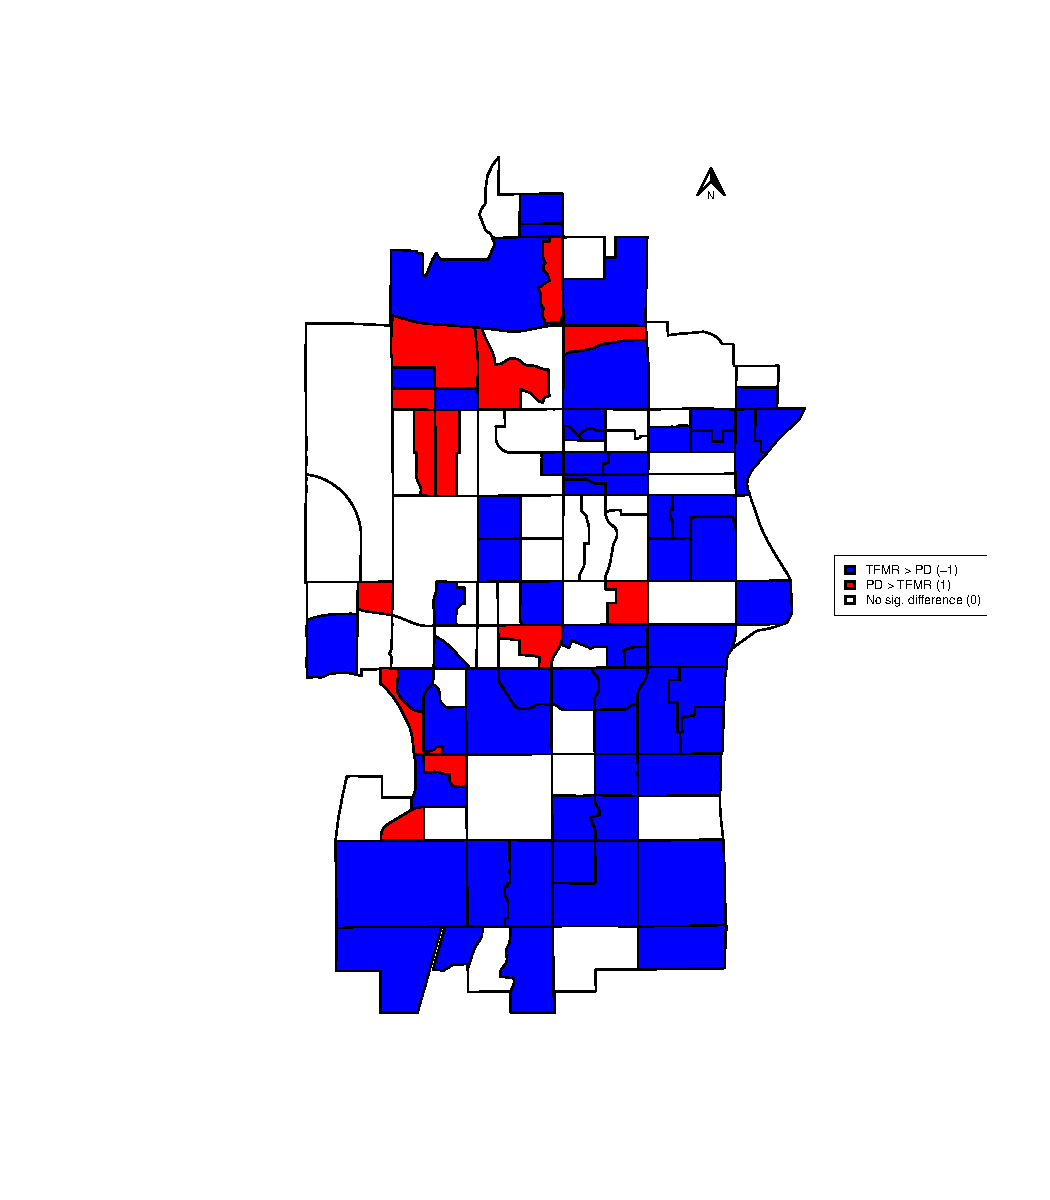
\includegraphics{figures/sppt-naloxone.pdf}
\end{figure}

\newpage

\begin{table}[htbp]\centering
\def\sym#1{\ifmmode^{#1}\else\(^{#1}\)\fi}
\caption{Mixed-effects Logistic Regression Models Predicting PD and TFMR first to Administer Naloxone}
\begin{adjustbox}{max width=\linewidth}\begin{tabular}{l*{2}{c}}
\toprule
                &\multicolumn{1}{c}{PD naloxone first}&\multicolumn{1}{c}{TFMR naloxone first}\\
\midrule
\emph{Independent variable}&                 &                 \\
Violent crime rate (per 1000)&0.997\sym{**} (0.001)        &1.001\sym{*} (0.001)        \\
\vspace{.05em} \\
Initial dispatch complaint (ref = Overdose/poisioning)&                 &                 \\
Health/medical related&0.684\sym{*} (0.104)        &1.326\sym{*} (0.182)        \\
Accidental injury&0.477 (0.502)        &0.770 (0.318)        \\
Public safety related&0.273 (0.282)        &0.519 (0.322)        \\
Mental health related&0.391\sym{**} (0.096)        &1.998\sym{**} (0.365)        \\
Other           &0.649\sym{**} (0.108)        &2.948\sym{**} (0.473)        \\
\vspace{.05em} \\
Female          &0.774 (0.127)        &1.126 (0.123)        \\
\vspace{.05em} \\
\emph{Block group predictors}&                 &                 \\
Violent crime spatial lag&1.008 (0.006)        &0.997 (0.004)        \\
Drug offense rate (per 1000)&1.007\sym{**} (0.002)        &0.994\sym{**} (0.002)        \\
Drug offense spatial lag&0.995 (0.007)        &1.005 (0.006)        \\
Opioid OD rate logged&0.937 (0.096)        &1.029 (0.087)        \\
Opioid OD spatial lag&0.996 (0.007)        &0.999 (0.006)        \\
\% Unemployed   &0.993 (0.012)        &0.999 (0.005)        \\
\% Residential land&1.001 (0.003)        &1.003 (0.002)        \\
\% Owner occupied units&0.978\sym{*} (0.009)        &0.995 (0.006)        \\
\% White        &1.012 (0.008)        &0.997 (0.005)        \\
\% Black        &1.025\sym{**} (0.007)        &0.987 (0.007)        \\
\% Hispanic     &1.007 (0.008)        &0.996 (0.006)        \\
Constant        &0.098\sym{**} (0.074)        &0.683 (0.355)        \\
\midrule
Random intercept&1.000\sym{**} (0.000)        &1.000 (0.000)        \\
\midrule
Observations    &     1,994        &     1,994        \\
Block groups    &  115        &  115        \\
AIC             & 1645.796        & 2464.457        \\
BIC             & 1830.527        & 2649.188        \\
\bottomrule
\multicolumn{3}{p{16cm}}{\footnotesize Exponentiated coefficients displayed. Clustered standard errors in parentheses. Month and year fixed effects included but not shown. Mean VIF value = 2.46, single highest VIF value = 7.49.}\\
\multicolumn{3}{l}{\footnotesize \sym{*} \(p<0.05\), \sym{**} \(p<0.01\), \sym{**} \(p<0.001\)}\\
\end{tabular} \end{adjustbox}
\end{table}


\newpage

\begin{figure}
    \caption{Coefficient Plot Predicting First to Administer Naloxone}
    \centering
    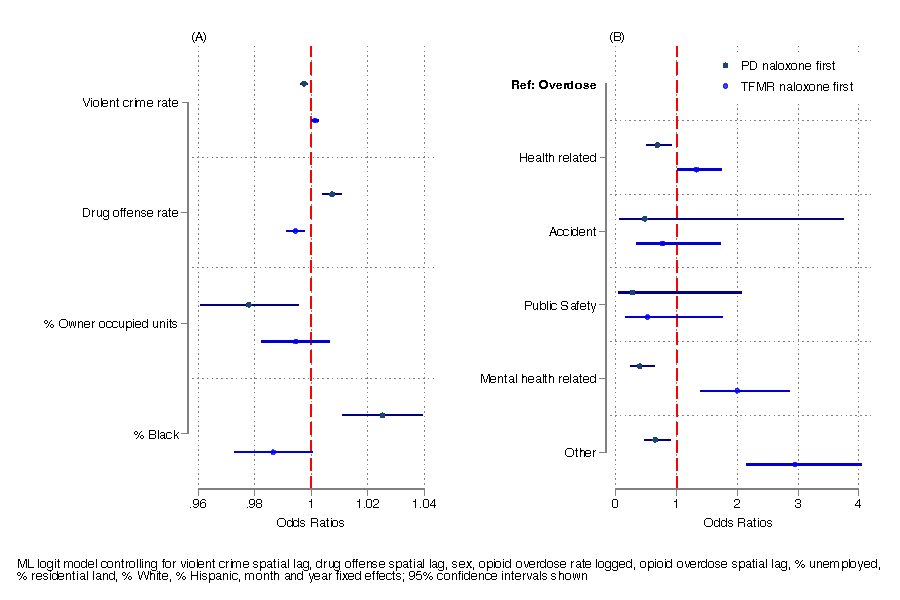
\includegraphics{figures/me-logit-coef-comb.pdf}
\end{figure}

\newpage 

\begin{table}[htbp]\centering
\def\sym#1{\ifmmode^{#1}\else\(^{#1}\)\fi}
\caption{Mixed-effects Logistic Regression Models Predicting PD and TFMR First to Administer Naloxone: PD and TFMR only}
\begin{adjustbox}{max width=\linewidth}\begin{tabular}{l*{2}{D{.}{.}{-1}}}
\toprule
                &\multicolumn{2}{c}{Police naloxone admin}\\\cmidrule(lr){2-3}
                &\multicolumn{1}{c}{(1)}        &\multicolumn{1}{c}{(2)}        \\
\midrule
\emph{Independent variable}&                 &                 \\
Violent crime rate (per 1000)&                 &0.995\sym{**} (0.001)        \\
\vspace{.05em} \\
Initial dispatch complaint (ref = Overdose/poisioning)&                 &                 \\
Health/medical related&                 &0.659\sym{*} (0.135)        \\
Accidental injury&                 &0.932 (1.005)        \\
Public safety related&                 &0.280 (0.193)        \\
Mental health related&                 &0.243\sym{**} (0.069)        \\
Other           &                 &0.347\sym{**} (0.072)        \\
\vspace{.05em} \\
Female          &                 &0.779 (0.149)        \\
\vspace{.05em} \\
Age range (ref = Aged 20 - 29)&                 &                 \\
Younger than 20 &                 &0.786 (0.279)        \\
Aged 30 - 39    &                 &0.881 (0.200)        \\
Aged 40 - 59    &                 &0.454\sym{**} (0.100)        \\
Aged 60 - 99    &                 &0.272\sym{**} (0.116)        \\
\vspace{.05em} \\
\emph{Block group predictors}&                 &                 \\
Violent crime spatial lag&                 &1.011 (0.007)        \\
Drug offense rate (per 1000)&                 &1.013\sym{**} (0.002)        \\
Drug offense spatial lag&                 &0.985\sym{*} (0.008)        \\
Opioid OD rate logged&                 &0.994 (0.149)        \\
Opioid OD spatial lag&                 &1.000 (0.001)        \\
Disadvantage&                 &1.079 (0.104)        \\
\% Residential land&                 &0.995 (0.003)        \\
\% Owner occupied units&                 &0.978 (0.013)        \\
\% White        &                 &1.024\sym{*} (0.011)        \\
\% Black        &                 &1.036\sym{**} (0.012)        \\
\% Hispanic     &                 &1.013 (0.010)        \\
Constant        &0.409\sym{**} (0.036)        &0.234 (0.263)        \\
\midrule
Random intercept&1.073 (0.067)        &1.000 (0.000)        \\
\midrule
Observations    &      955        &      891        \\
Block groups    &  112            &  106        \\
AIC             & 1170.921        & 1060.195        \\
BIC             & 1180.644        & 1381.282        \\
\bottomrule
\multicolumn{3}{p{20cm}}{\footnotesize Exponentiated coefficients; Clustered standard errors in parentheses; Day of month, month, and year fixed effects included but not shown; Mean VIF value = 2.30, single highest VIF value = 9.95. Reference group is now TFMR administering first -- Not all other observations.}\\
\multicolumn{3}{l}{\footnotesize \sym{*} \(p<0.05\), \sym{**} \(p<0.01\), \sym{**} \(p<0.001\)}\\
\end{tabular} \end{adjustbox}
\end{table}


\newpage
\begin{figure}
    \caption{Coefficient Plot Predicting First to Administer Naloxone: PD and TFMR only}
    \centering
    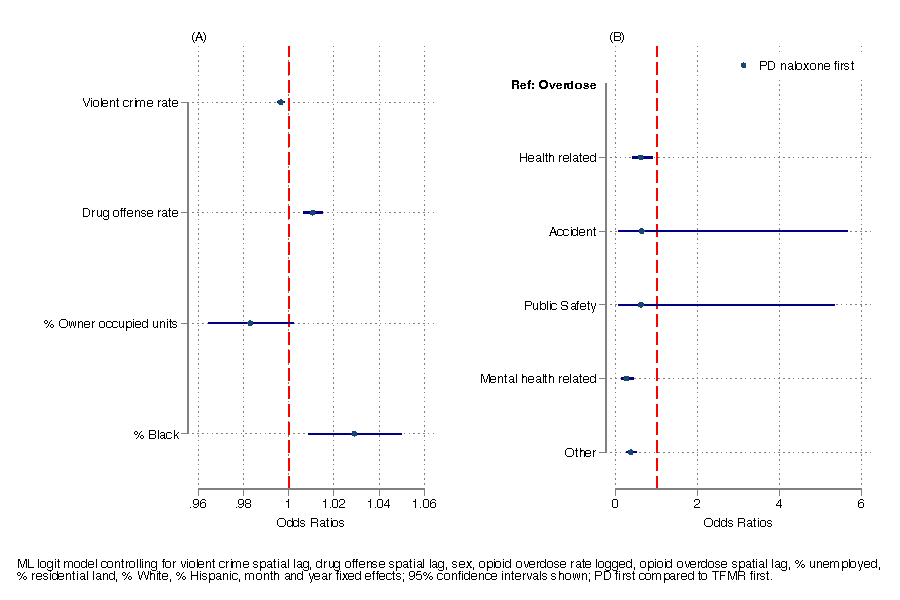
\includegraphics{figures/me-logit-coef-comb-sens.pdf}
\end{figure}
